This chapter consists of two sections, the first one shows an overview some of the
different methods that have been previously used in the literature
for understanding or quantifying urban perception.
The second section summarizes the main aspects of the research
on explainability on deep learning, and describes some techniques that have been applied
in urban perception or other domains that are relevant for this work.


\section{Understanding and quantifying urban perception.}

\subsection{Classic approaches.}
Methods for measuring perception of urban spaces have been part of the literature of several
disciplines for many years,  with some of the most influential studies dating back to 1960
\cite{lynch}. Due to technological limits the literature consisted mainly of different types of
qualitative surveys for a long time. These surveys consisted in having subjects complete
different tasks such as drawing maps of a certain place \cite{lynch}, evaluating fundamental
aspects of a neighborhood \cite{nasar_perception}, or in more recent approaches evaluating
the impact of transformations generated with edited images \cite{jiang_minimizing}. Most of
these surveys were conducted in person or by phone, and then the results were analyzed manually,
making it very difficult and costly to scale to multiple locations, or larger amounts of samples.
The main benefit of this approach, is that it allows for a precise control of the observation process
since both the subjects being interviewed and the spaces in question are chosen by the researcher.
Furthermore, the experiments conducted in person allow for the observer to use senses different
than vision to analyze the subject space, resulting in a richer appreciation.

A different methodology, more common in economics and engineering, consists of using discrete choice models
and stated choice surveys to model the effect of different variables in perception or other urban
related variables  \cite{rose_sc, iglesias_perception, torres_housing}. The amount and complexity of the
variables measured depends on the model design. To have and exact control of the variables that
have an effect on the survey, computer generated images of urban spaces can be used
\cite{iglesias_perception,torres_housing}.

The advantage of this method is that through the estimated parameters of the model, the effect
of each of the studied variables on the perception estimation can be measured, allowing for
quantitative results and an understanding of the impact different elements have on the
perception of the urban landscape. The main disadvantage of this approach comes from the
difficulty of the  survey design, variables need to be chosen carefully and the process its
vulnerable to biases from the model designer.

\subsection{Pure machine learning approaches.}

Thanks to the massive adoption of web and mobile technologies such as google maps, new types of
data are available in considerably large volumes, and new highly scalable ways of  generating data can be
designed and implemented quickly. That fact allows for some very data dependent machine learning
algorithms to be applied to new  problems, including urban perception estimation. Several different
datasets have been proposed for this problem, most of them based on surveys over large amounts of urban images
\cite{hidalgo_inequality, hidalgo_placepulse, quercia_aesthetic, liu_machine, santani}. The most important
of them, all consisting of pairwise comparisons of street view images, are \textit{Place pulse 1.0} (PP 1) \cite{hidalgo_inequality}
with measures of safety, class and uniqueness over images of 4 cities, \textit{Urban Gems} with measures of
beauty, quietness and happiness over images of London and \textit{Place pulse 2.0} (PP 2) \cite{hidalgo_placepulse}, the largest dataset
available, with measures of six different attributes over images of 56 different cities, the models proposed on this work are
trained on this dataset. All of these were collected through public online surveys of large scale, where the users
are asked to choose the image most representative of an attribute of a pair, see figure \ref{fig:survey} for an example.

\begin{figure}[ht]
	\begin{center}
	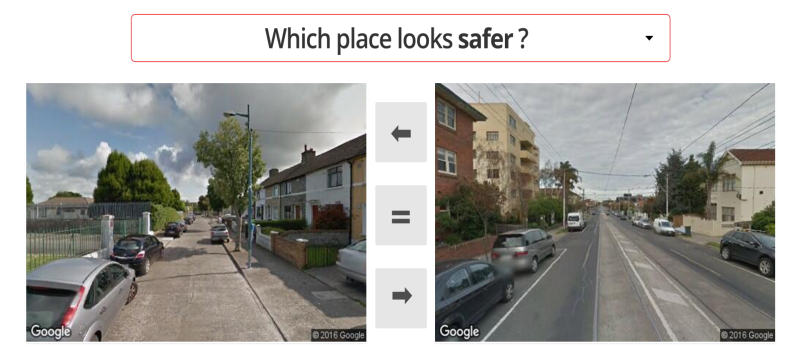
\includegraphics[width=0.5\textwidth]{./figures/placepulse.png}
	\caption[Place pulse 2.0 survey]{Snapshot of the place pulse 2.0 survey. Extracted from \citeA{hidalgo_placepulse} }
	\label{fig:survey}
	\end{center}
\end{figure}

Earlier attempts at using this data for training models tried to turn the problem into a classification problem
by  ranking the images from the votes with manually engineered methods such as the one suggested on the
place pulse 1.0 paper \cite{hidalgo_inequality} and use the rank to split the data in two halves with a different
label, \citeA{tamara_judgments} use this approach to train SVM models on PP 1 using different types of visual features as input,
including a deep neural network. On the PP 2 paper, the authors present the first end to end deep learning model for
urban perception regression, which uses a typical transfer learning technique \cite{survey_transfer}, a
Imagenet \cite{imagenet} pretrained  network for the base of the model, which is used as input
for by two parallel modules, one for classification and one for regression. They train the architecture
separately on the 6 different attributes of the dataset, the models learn to emulate human voting and
to output a urban perception score (through the regression module) on the image for the correspondent attribute.
Other works \cite{porzi_predicting, santani} take similar approaches but pretrain models or use features based on
the places dataset \cite{zhou_places}, which provides better performance according to their results.


\citeA{zhang_measuring}, train models on PP 2 by combining a DCNN features and a SVM classifier, they use this model to
obtain perception indicators of Beijing, they also use a semantic segmentation model \cite{cordts_cityscapes} on the images and used the results
as input to a linear regression, interpreting the regression weights as an indication of importance of the different segmentation
classes on perception. On a following work \cite{zhang_uncovering} they train one deep network to predict all 6 attributes of PP 2
in one forward pass, they do this using an end-to-end architecture similar to \citeA{hidalgo_placepulse} but adding
one output and loss component for each attribute.

Is important to note that most of the literature so far is more focused on applying the models to new cities
\cite{zhang_measuring, santani, costa_lisbon, rossetti} or generating new datasets with new attributes
\cite{santani, zhang_uncovering}, than it is on improving model  design and performance.
This is consistent with the fact that so far no good measures of performance for this problem have been defined,
due to the fact that the datasets don't provide a measure of perception per se but a proxy through the survey votes.
The objective of the models in the literature is to rank the images by the estimated perception of an attribute, but
they measure  performance using accuracy on classification of the human votes, which doesn't necessarily correlate with the
models capacity to generalize and rank well, especially in conflicted cases where even human voters
would have difficulties \cite{zhang_measuring}. Despite the fact that models in the literature don't surpass 70\%
classification  accuracy on  PP2, the actual ranking task seems to have correct results either by visual inspection,
or by comparing with metrics from other domains such as crime rates or wealth indicators \cite{rossetti,zhang_measuring,tamara_judgments}.


\subsection{Mixed approaches.}
\label{section:mixed}

With the intention of generating more or different insights, usually more explainability, some
work in the literature consists of combinations of computer vision or machine learning methods
with other techniques. In \citeA{rossetti} the authors use a combination of low and high level features
of the images as input for a discrete choice model that calculates perception. They extract low level features
with traditional computer vision methods like edges or blobs and the high level features with a pretrained
neural network for semantic segmentation. The semantic segmentation features allow for a posthoc analysis of
the results, the authors reach conclusions like "Images with more sidewalks were deemed to be
safer, livelier and wealthier, but less beautiful on average" and they present a table with the significance
of each of the segmentation classes in each of the six PP 2 attributes according to the discrete model parameters.
On a similar line, as was mentioned earlier \citeA{zhang_measuring} in addition to their main method, use
semantic segmentation features (they aggregate them by percentage of pixels on the image)
as an input for multivariate linear regression allowing for similar conclusions to those of \citeA{rossetti}
but using the beta coefficients (see figure \ref{fig:beta}).

\begin{figure}[ht]
	\begin{center}
	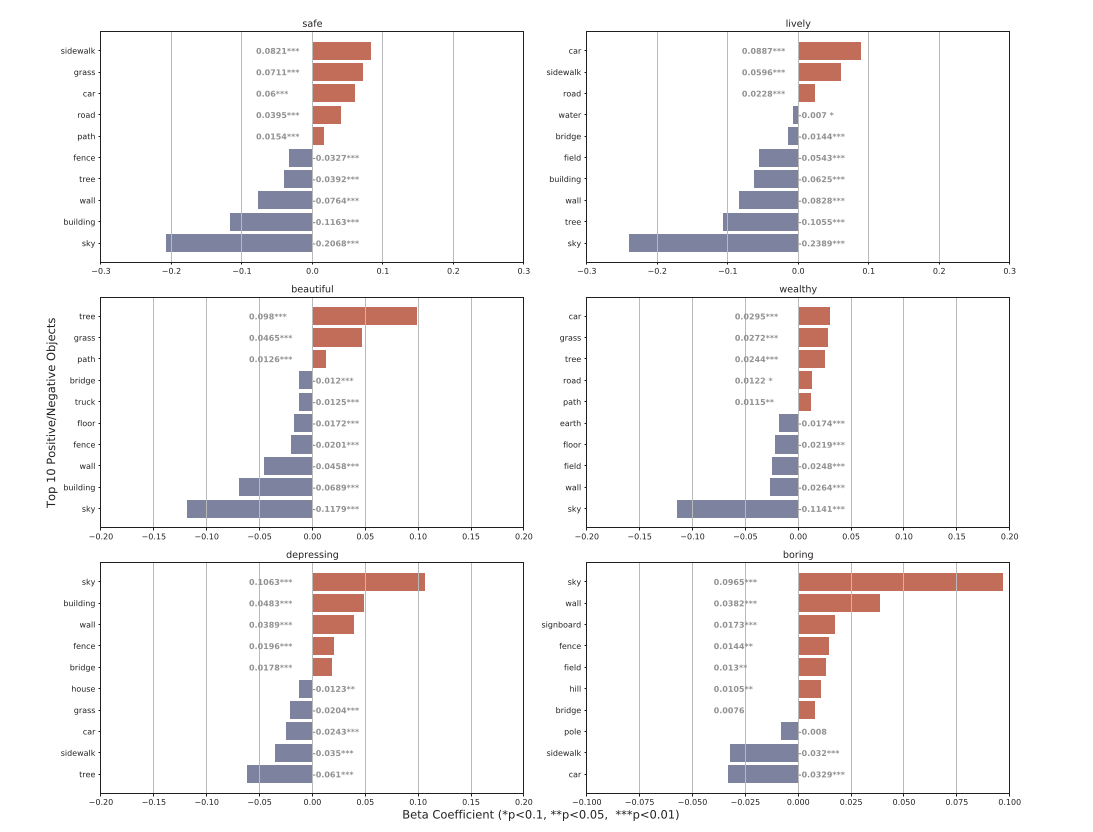
\includegraphics[width=1\textwidth]{./figures/zhang.png}
	\caption[Beta Coefficients]{ Linear regression beta coefficients for most significant objects. Extracted from \citeA{zhang_measuring} }
	\label{fig:beta}
	\end{center}
\end{figure}

On another work \citeA{seresinhe_beauty} train a DCNN to calculate the beauty of outdoor images,
using transfer learning from the Places dataset, but separately they use a places trained model to obtain text tags from
the scenes such as 'Mountain' or 'Tower', and similarly to \citeA{zhang_measuring} they use a regression model
(elastic net) to make conclusions about the significance of the concepts on the perception of beauty. The disadvantage
of this approaches is that they give more insights of the results only at a general level, and therefore do not allow for
conclusions on a per instance level, which is what this work intends to do.

Authors of \citeA{costa_lisbon} do an agreement analysis for this type of datasets,
they built their own dataset of pairwise comparisons for safety, but used it
for  generating clusters of users based on the semantic segmentation of the images they voted for.
They conclude that most clusters are due to lack of enough comparisons to do a good characterization
and that given enough votes all users converge to one generic profile. Is important to note
that authors don't provide any social or demographic information of the 439 users that
participated in the survey, and no other similar studies have been done so
far so their conclusion hasn't been replicated.

\section{ Explainability in machine learning.}

As was mentioned before, explainability has become a very active area of research
in machine learning, this is due to the large increase in the usage of ML models
for different day to day applications that affect the life's of thousands of people
\cite{ras_explanation}. For example, in cases where model outputs are used for analytics or decision
making, explainability can make the model both more trustworthy and informative.

\citeA{adadi_xai} summarize the reasons for enhancing explainability in four points:

\begin{enumerate}
	\item Explain to justify: To fullfil the need for reasons of a particular ML
	generated outcome.
	\item Explain to control: To allow a better handling of model behavior.
	\item Explain to improve: The additional understanding of model outputs is useful
	to design improvements on the systems.
	\item Explain to discover: As a model overcomes human performance in a task, if its
	doing so in an explainable manner, then new knowledge for humans may be obtainable.

\end{enumerate}

Is also important to note that laws and regulations related to this topic may become norm
in the future such as with the \citeA{gdpr}. According to it's articles
13, 14 and 15, when personal data is collected for automated decision-making,
the subject has the right to access, and the data controller is obliged to provide,
“meaningful information about the logic involved  as well as the significance and the envisaged
consequences of such processing for the data subject”, which will be very difficult to comply with,
when working with something like a black box neural network.

One of the two most common approaches to explainability in the literature are Post-hoc methods
\cite{adadi_xai} which try to obtain insights about how the models work, after the process of
inference over all the dataset is completed. The methods mentioned in section
\ref{section:mixed} are examples of this approach. Other more complex methods found in the recent literature
are based on analyzing model sensitivity to semantically meaningful concepts on input \cite{kim_tcav, shi_concept},
concepts that may be automatically mined from the data as in the approach proposed by \citeA{kim_ace}. This techniques, although
very promising, are still too recent and are not extensible to many domains.

The other approach, which is the one followed by this work, consists of taking advantage of the model
design to improve interpretability. This can be done by either using existent features of the model
or by introducing architectural changes that make them more explainable. A traditional  example of
this approach are rule based models like  decision trees \cite{breiman_tree}. Due to the black box
nature of deep neural networks this becomes a much more complex task for deep learning, and its an
important area of research.

Earlier solutions found in the literature consist of augmenting
model input with semantic information, such as text, object bounding boxes or even knowledge bases
\cite{dong_semantic, zhuo_video, li_knowledge}. This methods usually require additional supervision
which restricts them to densely annotated datasets such as Visual Genome \cite{krishna_visualgenome},
and the way the neural networks actually  use the additional information is not always clear.

Other very common technique in the literature is the use of attention based models \cite{bahdanau_attention},
which have layers that consist on using a part of the input (usually called query) to compute a set of weights
for the rest of the input (usually called value). The attention weights are usually computed through
a linear transformation and a softmax operation on the query, giving them the property of being a probability
distribution over the value vector \cite{cordonnier_relationship}, which is used to increase or decrease,
parts of the value vector and therefore the layer output. A particular case of attention is
self-attention, which means that the same vector is used as both query and input. A common attention architecture
in the recent literature is the transformer \cite{vaswani_attention}, which has been widely adopted in both
language and vision tasks \cite{devlin_bert, radford_gpt, bello_attention, li_visualbert, carion_object}.

Attention models have the additional value that the weights can be used to interpret what the network is doing, providing
explainable information about the model's decision process for each data instance \cite{wiegreffe_attention}.
\citeA{clark_bertlook} analyse the attention outputs of the NLP transformer model BERT and show how they correspond
well to linguistic notions of syntax, \citeA{zhang_interpretable} create an explainable VQA model by adding
supervised self-attention layers and visualizing their output as heatmaps over the input images
(see figure \ref{fig:vqa}). \citeA{cordonnier_relationship} present a theoretical  relationship between
between self attention and convolutional layers, and as part of their work they provide an interactive visualization
of the attention weights \footnote{Available at \url{epfml.github.io/attention-cnn/}}. \citeA{jiang_fantastic} present
a dataset that includes attention labels for images generated by human eye movement, allowing models to learn
correct human like attention patterns. Is clear that visualization of attention weights has become a prominent tool
for improving model explainability on the recent deep learning literature not only on language but on
vision tasks as well \cite{zhang_relation, johnston_depth, carion_object}.



\begin{figure}[ht]
	\begin{center}
	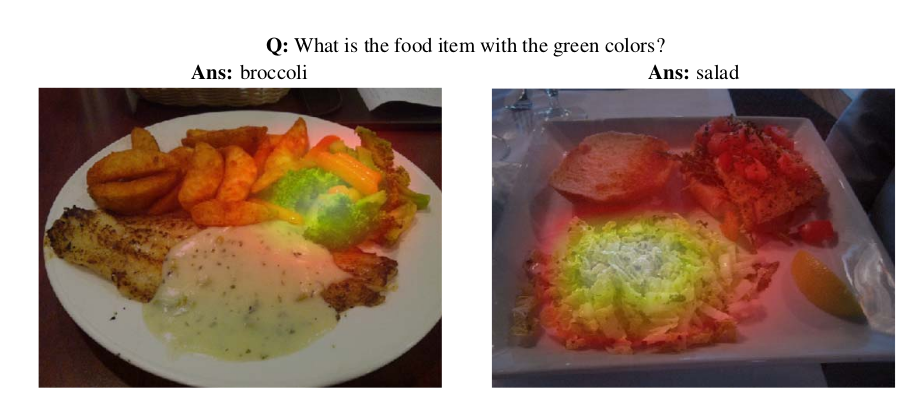
\includegraphics[width=0.8\textwidth]{./figures/soto.png}
	\caption[Attention on VQA]{Visualization of attention weights for the VQA problem. Extracted from \citeA{zhang_interpretable} }
	\label{fig:vqa}
	\end{center}
\end{figure}

